\chapter{Produktvorarbeit}
\section{Untersuchungen}
\subsection*{Pfaditechniken}

Der Inhalt der App werden die Pfaditechniken sein welche in sechs Themen Aufgeteilt sind: Pionier, Karte und Kompass, Übermittlung, Natur und Umwelt, Samariter und Pfadigeschichte. Alle wichtigen Informationen zu diesen Themen werden unten erläutert.

\subsection*{Pionier}

Bei Pionier geht es rund um Seile, Knoten, Blachen und Zelte. Dabei ist wichtig, dass es nicht nur darum geht wie man sie benutzt sondern auch wie man sie Pflegt und was sie für Vorteile und Nachteile mit sich bringen.

\subsubsection*{Seile}

Bei den Seilen unterscheidet man zwischen vier Seilarten, Hanfseile, Bergseile, Statikseile und Polypropylenseile. Polypropylenseile sind dabei für Pionierarbeiten zu vernachlässigen, da diese schnell schmelzen. Die anderen Seilarten haben folgende Eigenschaften:
\begin{center}
\begin{tabularx}{\textwidth}{p{0.2\textwidth}|X|X|X}
     & \textbf{Hanfseil} & \textbf{Bergseil} & \textbf{Statikseil} \\ \hline
     Bild & 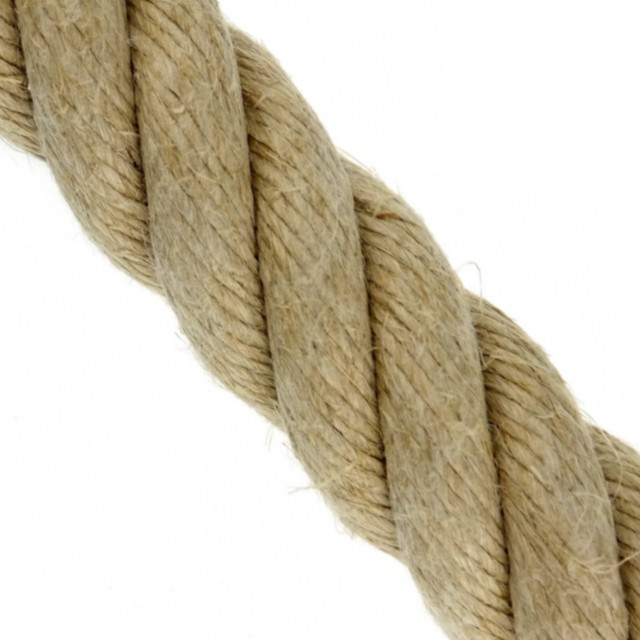
\includegraphics[width=0.2\textwidth]{Picture/hanfseil.png} & 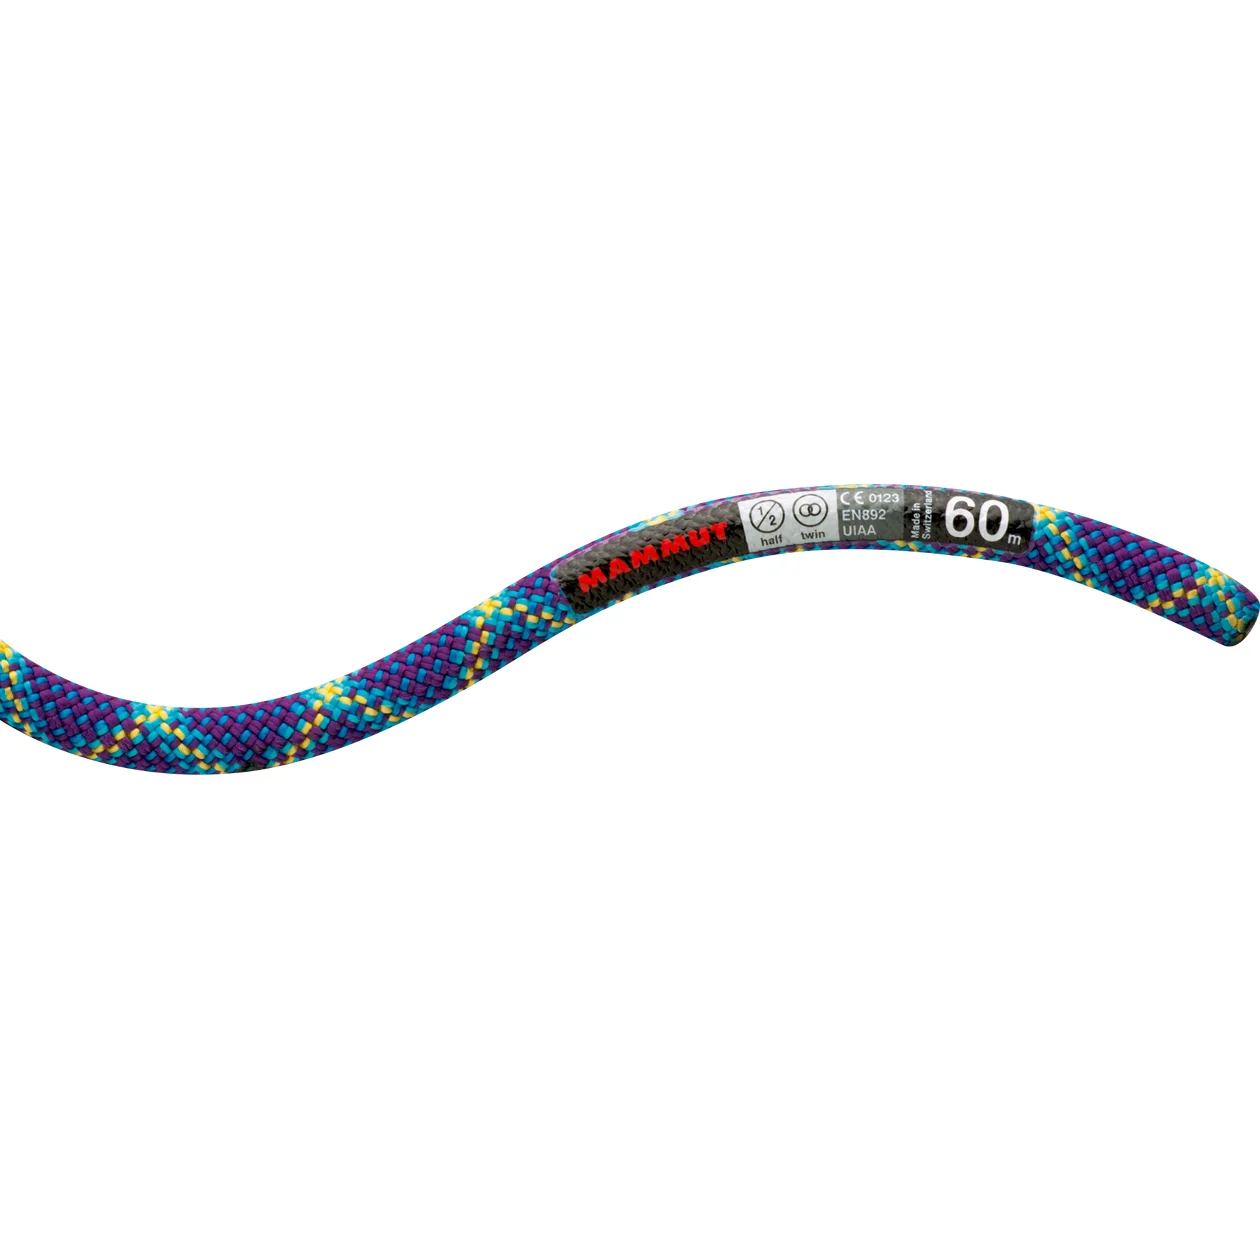
\includegraphics[width=0.2\textwidth]{Picture/bergseil.png} & 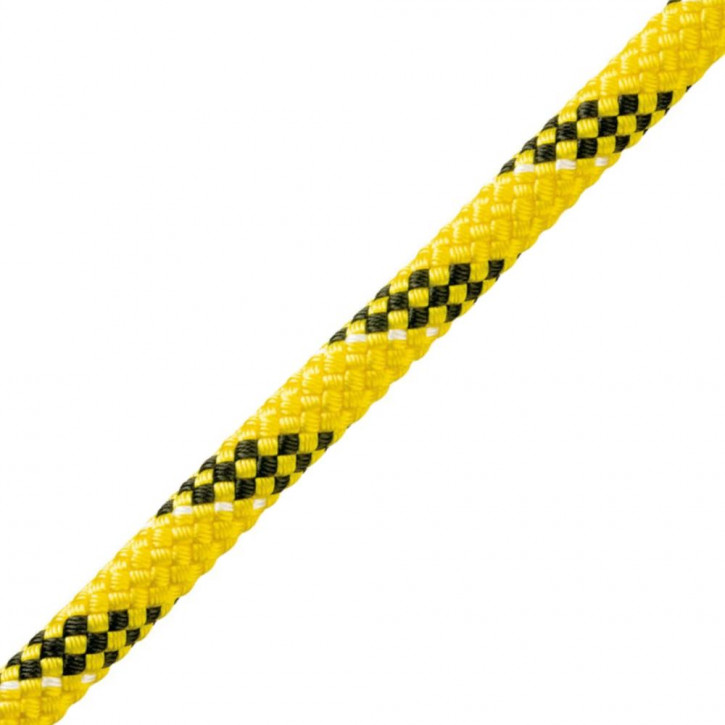
\includegraphics[width=0.2\textwidth]{Picture/statikseil.png} \\\hline
     Merkmal & braun, gedreht & farbig, geflochten & farbig, geflochten \\\hline
     Anwendung & Pioniertechnik, Seilbrücken & Abseilen & Seilbahnen, Strickleiter \\\hline
     Dehnung & gering & gross & gering \\\hline
     Temperatur- beständigkeit & $\approx$ 200$^\circ$C & $\approx$ 100$^\circ$C & $\approx$ 100$^\circ$C \\\hline
     Reissfestigkeit (trocken 10mm) & 800 kg & 2000 kg & 3000 kg \\\hline
     Material & Naturfaser & Kunstfaser (Nylon, Polyamid) & Kunstfaser (Nylon) \\\hline
     Scheuerfestigkeit & gut & empfindlich & gut \\\hline
     Verrotungs- beständigkeit & schlecht & gut & gut \\\hline
     Wasseraufnahme & viel (verkürzt sich) & wenig & wenig \\
\end{tabularx}
\end{center}
Die Seilpflege ist ein weiterer sehr wichtiger Aspekt wenn es um Seile geht, damit diese noch lange halten und auch sicher für den Gebrauch sind. Die fünf wichtigsten Sachen hierbei sind:

\begin{enumerate}
    \item Stehe nicht auf Seile
    \item Reinige Seile regelmässig (trocken)
    \item Schütze Seile vor Schmutz, Feuchtigkeit und direkter Sonnenbestrahlung
    \item Lagere Seile trocken und vor Sonnenlicht geschützt
    \item Lasse Seile nie über scharfe Kanten laufen
\end{enumerate}

\subsubsection{Knoten}

Genau wie bei den Seilen gibt es auch bei den Knoten einige Sachen auf die man achten sollte wenn man einen macht:
\begin{itemize}
    \item Befestige alle Knoten
    \item Ein Knoten halbiert die Tragfähigkeit eines Seiles
    \item Lasse am Knotenende genügend freies Seil
    \item Bringe einen Stecken beim Knoten in zwischen die Verbindung um den Knoten nach der Belastung wieder öffnen zu können.
\end{itemize}

Nun aber zu einer Tabelle mit den wichtigsten Knoten und ihren Eigenschaften:
\begin{center}
\begin{tabularx}{\textwidth}{X|X|X|X|X}
    \textbf{Name} & \textbf{Bild} & \textbf{Verwendung} & \textbf{Positive Eigenschafte} & \textbf{Negative Eigenschaften} \\\hline
    Samariter & & Verbindung gleich dicker Seile & Einfach, Flach, leicht straffzuziehen & Öffnet sich bei grosser Belastung \\\hline
    Weber & & Verbindung ungleich dicker Seile & Einfach zu knöpfen, leicht straffzuziehen & Öffnet sich bei grosser Belastung\\\hline
    Fischer/ Spierenstich & & Verschiebbare Verbindung zweier ungleich dicker Seile & Hält sicher, kleine verringerung der Reissfestigkeit & Schwer zu öffnen \\\hline
    Gesteckter \footnote{Kann um einen Baum geknöpft werden} Achter& & Schlinge zum Anseilen & Hält sicher, gut zum Öffnen & - \\\hline
    Bretzeli & & Seilbefestigung an dünnen Gegenständen & Schnell geknöpft & Mühsam zu öffnen \\\hline
    Maurer & & Seilbefestigung an dicken Gegenständen & Einfach zu öffnen & Nur eine Zugrichtung, Hält nur bei Belastung \\\hline
    Fläschli/Päckli & & Zulaufende Schlinge für Pakete, Spanner, Strickleitern & Einfach zu knöpfen & Nur eine Schlaufen und Zugrichtung, mühsam zum öffnen \\\hline
    Fuhrmann & & Zulaufende Schlinge für Spanner & Besser lösbar als Flächli/Päckli & Nur eine Schlaufen und Zugrichtung, mühsam zum öffnen \\\hline
    Anker & & Befestigung einer Schlaufe & Einfach zu knöpfen & Seitliches verrutschen, gleicher Zug an beiden Enden \\\hline
    Halbmastwurf & & Abseilen von Lasten & Gute Kontrolle von Lasten & Schnell falsch geknöpft, schwere Handhabung \\\hline
    Achterschlinge/ Mastwurf & & Fixieren eines Seiles & Hält sehr gut, schräger Zug möglich & Mühsam zu öffnen \\\hline
    Schachbrett-/Freundschafts- knoten & & Zierknoten zum Binden der Pfadikrawatte & Flacher Knoten & Mühsam zu öffnen \\
\end{tabularx}
\end{center}

\subsection*{Programmiersprache Java}


\subsection*{Aufbau Android App}



\subsection*{GitHub}